\chapter{深度学习以及其不确定性量化简介}

深度学习通过构建多层非线性变换网络实现对数据特征的层次化抽象,
已成为现代人工智能的核心范式。本章在\ref{intro-NN}节中介绍了神经网络的基础架构,
阐述深度学习的基础理论框架,重点解析神经网络的结构特性与训练机制,
在\ref{transformer}节深入探讨了Transformer模型的自注意力机制,
并在\ref{uncertainties}节全面论述了不确定性量化的前沿方法与技术挑战。

\section{神经网络基础架构简介}\label{intro-NN}

神经网络是一种模拟人脑神经元结构和功能的计算模型。它由大量的神经元通过连接权重相互连接而成。
神经网络跟生物上的神经系统类似,其基本单元都是神经元,每个神经元接收来自其他神经元的输入信号,
并在神经元之间通过激活函数引入非线性关系将其转换为输出信号。
神经网络的学习过程就是通过调整连接权重来最小化预测值与真实值之间的误差。
一般来说,一个简单的神经网络的结构通常分为输入层、隐藏层和输出层。
输入层接收从外界输入的数据,接着经过处理之后传递到隐藏层,
同时通过激活函数对输入数据进行非线性变换,
最后输出层会将隐藏层的输出转换为最终的预测结果 (通常为点估计) 。
神经元的输出信号可以表示为:
\begin{equation}
  A_{i,j} = F\left(\sum_{k=1}^{n} W_{i,j,k} X_k + B_{i,j}\right)
\end{equation}
其中,$A_{i,j}$为第$i$个神经元在第$j$层的输出信号,
$W_{i,j,k}$为第$i$个神经元在第$j$层与第$k$个神经元在第$j+1$层的连接权重,
$B_{i,j}$为第$i$个神经元在第$j$层的偏置项,$F$为激活函数,用于引入非线性变换。
常用的激活函数有sigmoid函数、反正切(tanh)函数和ReLU(rectified linear unit,整流线型单元)函数等。
其中sigmoid和tanh函数呈S型曲线,一般来说更适用于二分类问题;而ReLU函数则是一种分段线性函数,
在多分类问题中具有很不错的表现。
图\ref{NNstructure}展示了一个简单的神经网络结构,其中包含一个输入层、两个隐藏层和一个输出层。

\begin{figure}[htbp]
  \centering
  \begin{tikzpicture}[x=2cm,y=2cm] % 调整了y的值以增加垂直间距
    \usetikzlibrary{fit}
    \readlist\Nnod{2,3,3,2} % 输入层2个node,两个隐藏层每层3个node,输出层2个node
    \foreachitem \N \in \Nnod { % loop over layers
      \foreach \i [evaluate={\x=\Ncnt; \y=\N/2-\i+0.5; \prev=int(\Ncnt-1);}] in {1,...,\N} { % loop over nodes
      % 根据不同层添加不同的标签
      \ifnum\Ncnt=1
        \node[mynode, fill=blue!40](N\Ncnt-\i)at(\x,\y){$x_{\i}$};
      \else
        \ifnum\Ncnt=\Nnodlen
        \node[mynode, fill=red!40](N\Ncnt-\i)at(\x,\y){$y_{\i}$};
        \else
        \node[mynode, fill=green!40](N\Ncnt-\i)at(\x,\y){$a_{\the\numexpr\Ncnt-1\relax,\i}$};
        \fi
      \fi
      % 为连接的线加上标签,只在输入层到第一个隐藏层中,当连接来自x1时添加对应数字的权重标签
      \ifnum\Ncnt>1
        \pgfmathsetmacro{\prevCount}{\Nnod[\prev]}
        \foreach \j in {1,...,\prevCount} {
        \ifnum\Ncnt=2
          \ifnum\i=1
          \ifnum\j=1
            \draw[thick](N\prev-\j)-- node[midway, above] {$\omega_{1,1,1}$}(N\Ncnt-\i);
          \else
            \draw[thick](N\prev-\j)--(N\Ncnt-\i);
          \fi
          \else
          \draw[thick](N\prev-\j)--(N\Ncnt-\i);
          \fi
        \else
          \draw[thick](N\prev-\j)--(N\Ncnt-\i);
        \fi
        }
      \fi
      }
      % 绘制层的虚线边框
      \ifnum\Ncnt=1
        \def\LayerColor{black}
      \else
        \ifnum\Ncnt=\Nnodlen
          \def\LayerColor{black}
        \else
          \def\LayerColor{black}
        \fi
      \fi
      \node[draw=\LayerColor, dashed, rounded corners, inner sep=5pt, fit=(N\Ncnt-1)(N\Ncnt-\N)] {};
      % 添加层的标签
      \ifnum\Ncnt=1
      \node[below] at(\Ncnt,-1.5){输入层};
      \else
      \ifnum\Ncnt=\Nnodlen
        \node[below] at(\Ncnt,-1.5){输出层};
      \else
        \node[below] at(\Ncnt,-1.5){隐藏层};
      \fi
      \fi
    }
    \end{tikzpicture}
  \caption{神经网络基本结构的示意图,这里包含输入层、两个隐藏层和输出层,每个隐藏层的神经元都被连接到前一层的所有神经元。
  最后的输出层将隐藏层的输出转换为最终的预测结果,在训练过程中,最终的输出结果会与真实值进行比较,从而计算损失函数。}
  \label{NNstructure}
\end{figure}

神经网络在训练中通常采用反向传播算法,
该算法通过计算并降低损失函数的梯度来更新连接权重。
损失函数为训练中最重要的部分,其选择几乎决定了模型训练的效率和效果。
其功能主要为量化预测值与真实值之间的差距,
常见的损失函数包括均方误差和交叉熵等。在模型的训练过程中,
我们通常使用梯度下降算法不断迭代,从而做到优化这些权重,
进而可以使损失函数被最小化并找到最优参数,
其数学本质为参数空间的最速下降过程:

\begin{equation}
  \theta = \arg\min_{\theta} \mathcal{L}(f_\theta(x), y)
\end{equation}
其中,$\theta$为神经网络的参数,$\mathcal{L}$为损失函数,$f_\theta(x)$为神经网络的预测函数,$y$为真实值。


上面介绍的神经网络是属于前馈神经网络。基于前馈网络的深度学习模型有很多类型,
其中最常见的包括卷积神经网络(CNN,convolutional neural network)和循环神经网络(RNN,recurrent neural network)。
CNN最初被设计用于图像处理任务,其核心思想是通过卷积层自动提取图像的局部空间特征,
并利用池化层进行特征降维和抗干扰。卷积层能够有效捕捉图像中的边缘、
纹理等低级特征,如果我们把网络层数加深加多,还能更有效地逐步提取更复杂的抽象特征。
池化层则通过下采样操作减少特征图的尺寸,从而降低模型参数量和计算复杂度,
同时有助于缓解过拟合问题。相比之下,循环神经网络(RNN)则专为处理序列数据而设计。
RNN通过在时间步之间传递隐藏状态,实现对序列中前后依赖关系的建模。
为了解决传统RNN在长序列训练中易出现的梯度消失或爆炸问题,研究者提出了LSTM(long short-term memory,长短时记忆)\cite{hochreiter1997long}
或GRU (gated recurrrent unit,门控循环单元) \cite{DBLP:journals/corr/ChoMGBSB14}这样的方法,
特别是用来解决序列中长距离依赖的问题。
虽然卷积神经网络和循环神经网络都是深度学习的重要部分,
但传统的RNN在处理长序列时常常效率不高,还容易遇到梯度消失或爆炸的问题。
因此,除了LSTM和GRU这些改良的RNN之外,后续介绍的Transformer模型也在广泛应用中。

\section{Transformer}\label{transformer}

Transformer是一种基于自注意力机制的神经网络模型,
最早由Google在2017年提出\cite{vaswani2017attention}。
这个模型的最大特点是利用自注意力机制,能够捕捉序列中不同位置之间的关系,
因此特别擅长处理序列数据,比如翻译、文本生成等。整个Transformer由两个主要部分组成:
编码器和解码器。编码器的任务是把输入序列变成一个包含上下文信息的向量,
解码器则根据这个向量和之前生成的内容,逐步生成输出序列。这两部分都是由多个相同的层叠加而成,
每一层都包含多头注意力机制和前馈神经网络。编码器和解码器之间会通过交叉注意力连接,
让模型更好地理解输入和输出的关系。具体来说,编码器的输入是一个序列,
经过多次注意力和前馈网络后,输出一个总结整个输入的上下文向量。
而解码器除了会用到这个上下文向量,还会结合之前生成的内容,经过层层处理,
预测下一步的输出。最终,解码器的输出经过线性变换和Softmax函数,
就能得到每个位置对应的概率分布。接着,可以用采样或贪心搜索等方法,
从这些概率中生成最终的输出序列。最后,图\ref{transformer}
展示了Transformer的整体架构。

\begin{figure}[htbp]
  \centering
  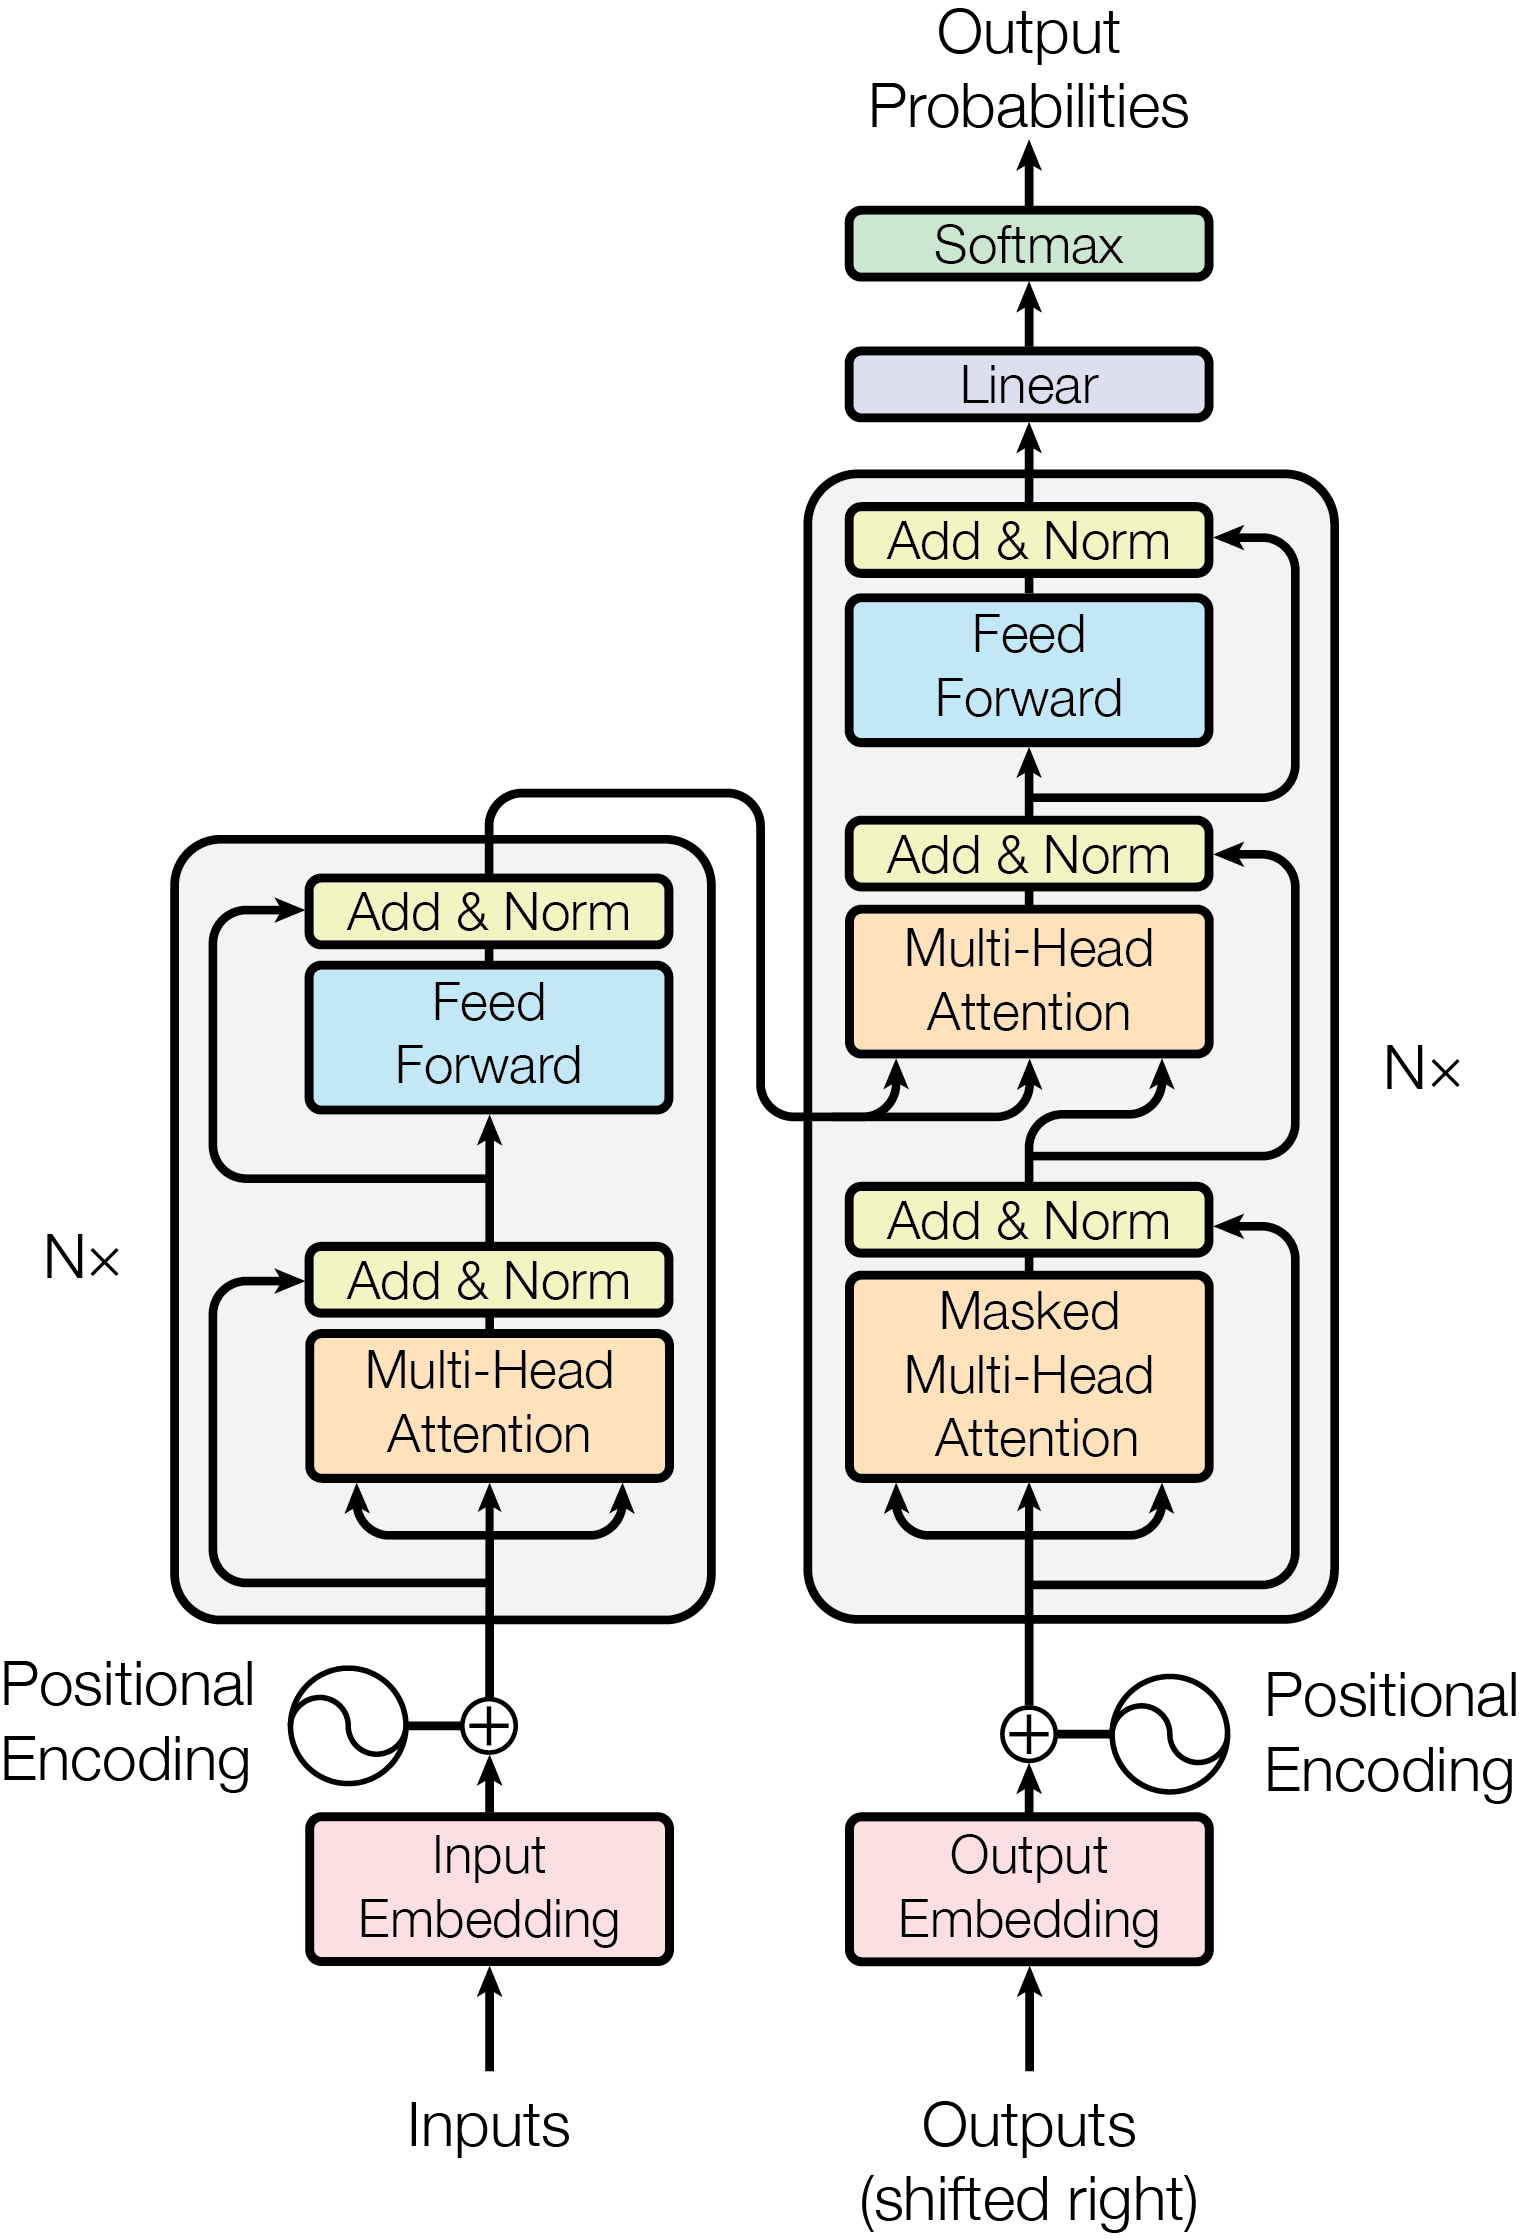
\includegraphics[width=0.45\textwidth]{figures/transformer.png}
  \caption{Transformer模型的基本结构示意图\cite{vaswani2017attention}}
  \label{transformer}
\end{figure}

\subsection{注意力机制}
注意力机制是一种能够动态分配不同输入位置权重的方法,这个机制主要
用于建模并量化序列中各个元素之间的关系。这个机制的核心思想是根据输入序列中各位置之间的相关性,
为每个位置分配不同的注意力 (权重) ,从而生成包含全局信息的上下文表示。
更具体的来说,注意力机制通常包括以下步骤:
首先计算查询(Query)与键(Key)之间的相似度,得到注意力权重\cite{vaswani2017attention}:
\begin{equation}
  \label{attention}
  \text{Attention} = \text{softmax}\left(\frac{QK^T}{\sqrt{d_k}}\right)
\end{equation}
其中,$Q$为查询 (Query) 矩阵,$K$为键 (Key) 矩阵,$d_k$为键矩阵的维度。
然后利用这些权重对值(Value)进行加权求和,形成上下文向量;
最后将上下文向量与原始输入结合,作为后续网络层的输入。
通过这种方式,模型能够灵活地调整,
从而寻找出与当前任务最相关的信息,有效提升对长序列数据的建模能力。

上面分析的注意力机制被称为“缩放点积注意力 (Scaled dot-product attention) ”,
不过我们从图\ref{transformer}可以看出,
进行应用的是“多头注意力(Multi-head attention)”。
这是由多个缩放点积注意力经过投影$h$次然后经过
$d_k$,$d_k$和$d_v$并行运算最后叠加而成的。
这一机制使得模型可以结合多个不同投影子空间的表现,从而获得更高精确度的预测。
为这两种注意力机制的示意图由图\ref{fig:multi-head-att}给出,
其中缩放点积注意力由公式\ref{attention},
而多头注意力用公式表征如下\cite{vaswani2017attention}:

\begin{align}
  \mathrm{MultiHead}(Q, K, V)&= \mathrm{Concat}(\mathrm{head_1}, ..., \mathrm{head_h})W^O\\
  \text{其中}~\mathrm{head_i} &= \mathrm{Attention}(QW^Q_i, KW^K_i, VW^V_i)\\
\end{align}

其中这些投影为参数矩阵$W^Q_i \in \mathbb{R}^{d_{model} \times d_k}$, $W^K_i \in \mathbb{R}^{d_{model} \times d_k}$, $W^V_i \in \mathbb{R}^{d_{model} \times d_v}$ and $W^O \in \mathbb{R}^{hd_v \times d_{model}}$.
\begin{figure}[htbp]
  \centering
  \begin{minipage}[t]{0.4\textwidth}
    \centering
    \vspace{0.5cm}
    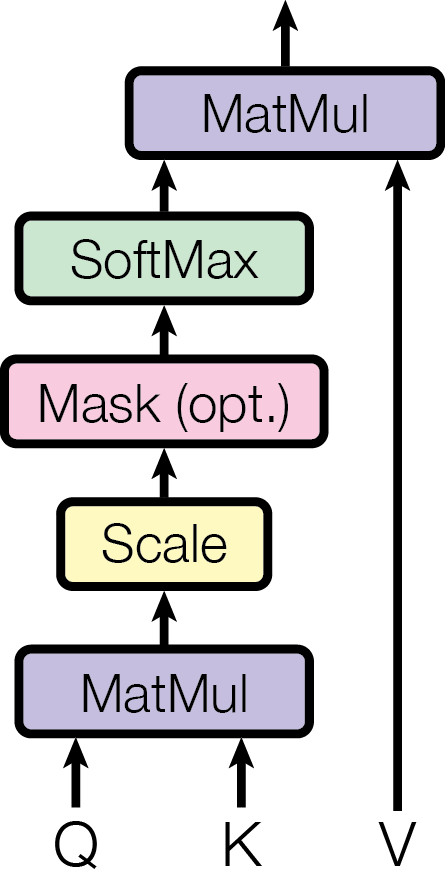
\includegraphics[scale=0.6]{figures/dotproductattention.png}
  \end{minipage}
  \begin{minipage}[t]{0.4\textwidth}
    \centering
    \vspace{0.1cm}
    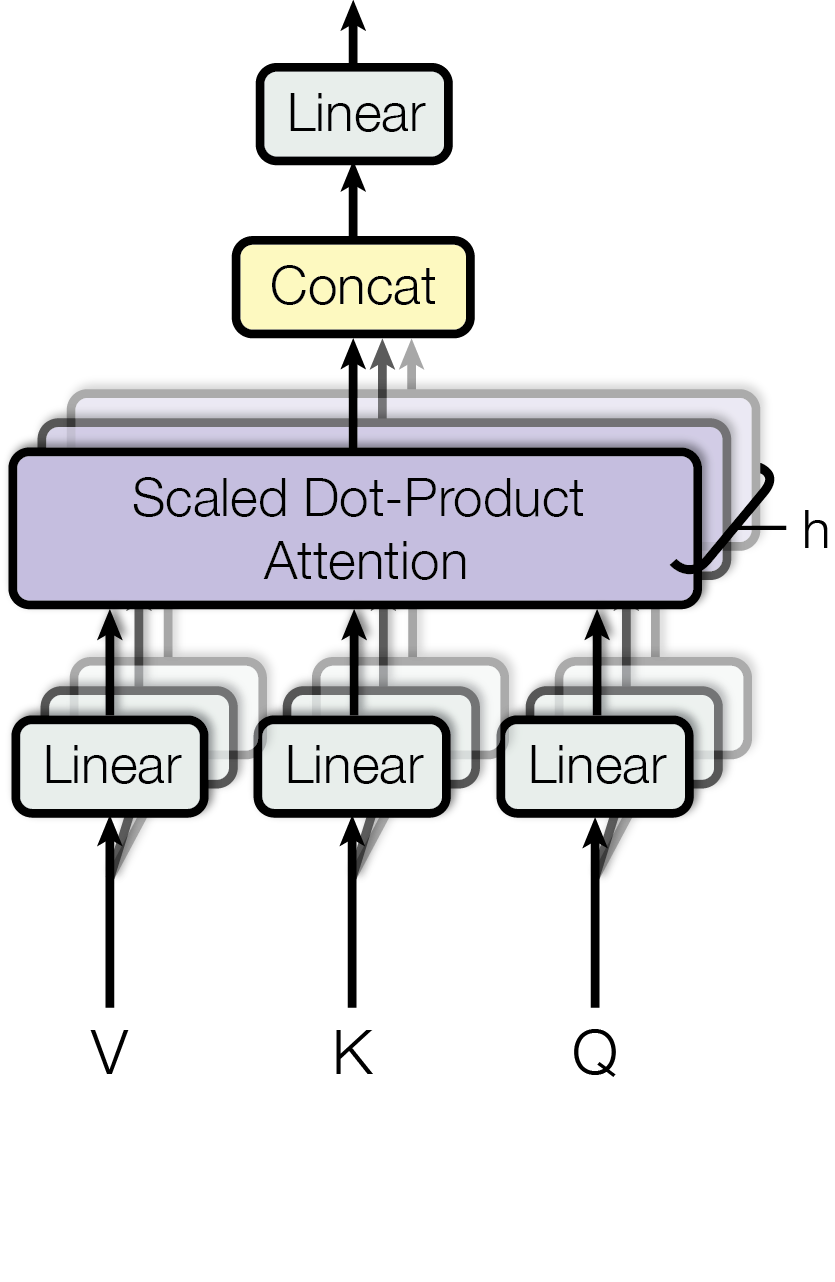
\includegraphics[scale=0.6]{figures/multihead.png}
  \end{minipage}
  \caption{左图为缩放点积注意力,右图为多头注意力由多个并行运行的缩放点积注意力层组成。\cite{vaswani2017attention}}
    \label{fig:multi-head-att}
\end{figure}

总而言之,Transformer模型通过其核心的自注意力机制,特别是多头注意力变体,
有效地捕捉了序列数据中的长距离依赖关系。其编码器-解码器架构,
结合位置编码和前馈网络,使其在序列到序列任务中取得了显著成功,
并成为现代深度学习模型的重要基石。


\section{深度学习中的不确定性分析}\label{uncertainties}
深度学习模型在各种领域展现出了强大的预测能力,
然而对这些模型预测结果的不确定性进行量化是一个重要且具有挑战性的问题。
不确定性量化(Uncertainty Quantification,UQ)旨在评估和表征
深度学习模型预测的可靠性和置信度。在实际应用中,
了解模型预测的不确定性对于决策制定、风险评估和模型解释至关重要。

在深度学习领域,不确定性可分为认知不确定性(模型不确定性)和随机不确定性(数据不确定性)。\cite{ABDAR2021243}
前者源于模型参数的不确定性,可通过贝叶斯方法量化;后者源于数据本身的噪声或随机性,
通常通过概率分布建模。深度学习中的不确定性量化方法主要包括BNN
(Bayesian neural network,贝叶斯神经网络)、
深度集成方法\cite{NIPS2017_9ef2ed4b}和MC(Monte Carlo,蒙特卡洛) dropout等技术。
这些方法使我们能够对模型预测结果提供可靠的不确定性估计,
从而增强模型在实际应用中的可靠性和可解释性。

\subsection{BNN}
BNN 的核心思想是将神经网络的权重 ($\omega$) 和偏置视为概率分布,
而不是固定的点估计值,如图\ref{bnn}所示。其目标是根据观测数据$D$推断权重的后验分布 $p(w|D)$ 。
对于新的输入 $x^*$,
BNN 的预测是通过对所有可能的权重配置进行边缘化(或积分)得到的,
即进行贝叶斯模型平均:\cite{ABDAR2021243}

\begin{equation}
    p(y^*|x^*,D) = \int p(y^*|x^*,w)p(w|D)dw
\end{equation}

\begin{figure}[htbp]
    \centering
    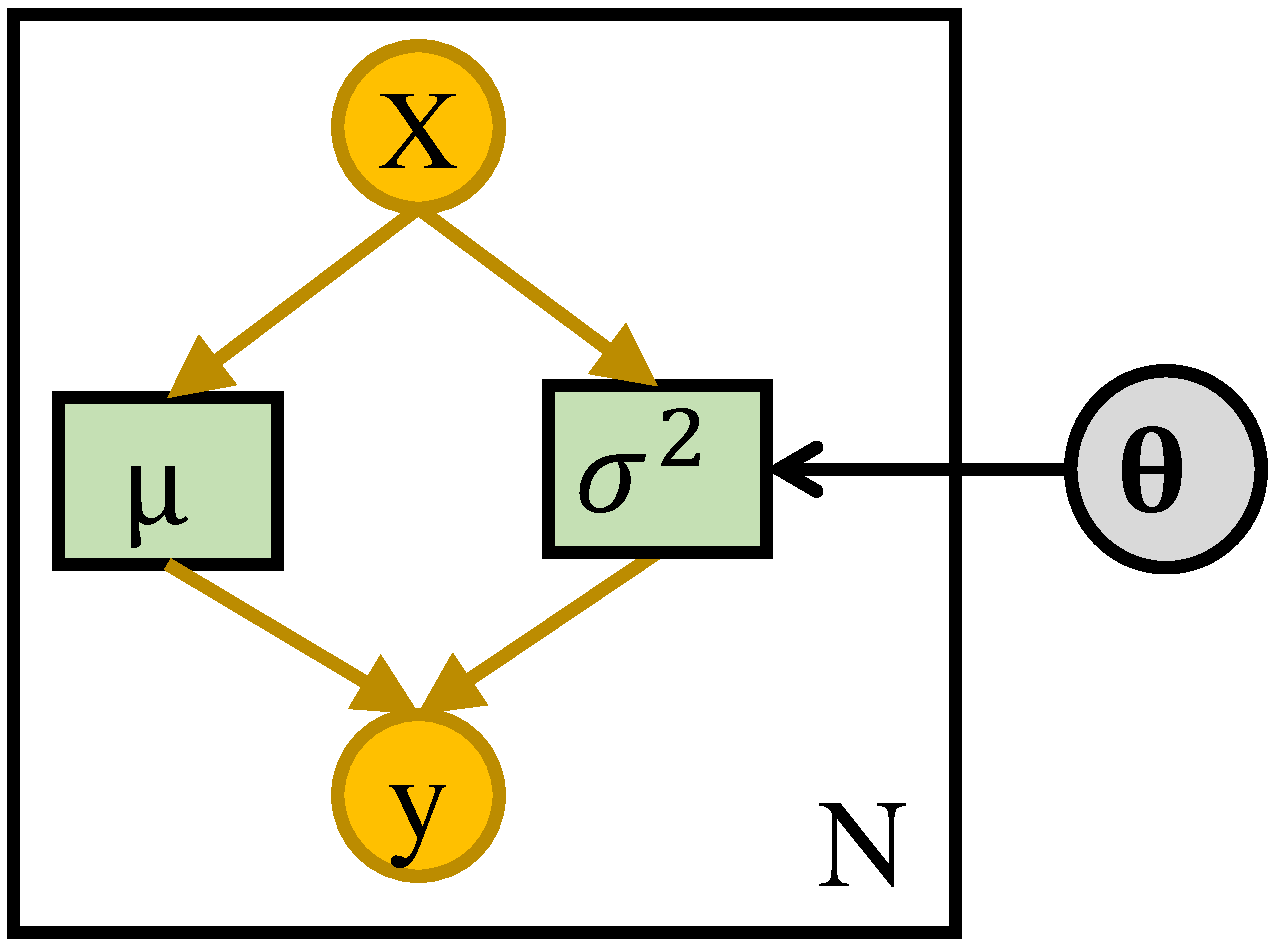
\includegraphics[width=0.45\textwidth]{figures/Bayesianneuralnetwork.pdf}
    \caption{贝叶斯神经网络的基本结构示意图\cite{DBLP:journals/corr/abs-2011-06225}}
    \label{bnn}
\end{figure}
由于精确计算后验分布通常是不可行的,我们一般
需要采用一些近似推断方法,
例如VI (Variational Inference,变分推断) ,
MCMC (Markov Chain Monte Carlo,马尔可夫链蒙特卡洛) ,拉普拉斯近似
等。

对于VI,我们使用一个简单的、可处理的概率分布
$q(\theta)$ (例如,均值场高斯分布) 来近似真实的后验分布
$p(w|D)$,通过最小化它们之间的Kullback-Leibler散度\cite{1320776d-9e76-337e-a755-73010b6e4b64}来优化近似分布的参数
。VI在计算上通常比MCMC更高效,但其结果依赖于近似分布的选择。

对于MCMC,我们通过构建马尔可夫链来从后验分布中采样。
MCMC一般被认为能够提供更加精确的估计,
但计算成本非常高,尤其对于参数量巨大的深度神经网络。

对于拉普拉斯近似,我们将后验分布近似为以最大后验概率
(MAP)估计为中心的高斯分布,其协方差矩阵由损失函数的
Hessian矩阵的逆给出。

BNN能够自然地捕捉认知不确定性(通过权重分布的方差体现)。
如果模型被设计为预测输出的分布参数
(例如,预测高斯分布的均值和方差),则也可以捕捉偶然不确定性。
一些研究工作尝试利用 BNN 来分离统计不确定性和系统不确定性。
一方面,BNN提供了严谨的贝叶斯框架;
有潜力产生良好校准的不确定性估计;
能够捕捉模型参数之间的复杂相关性。
不过另一方面,BNN计算成本高昂(尤其是MCMC);
结果可能依赖于先验分布的选择;而
VI的近似质量可能受限;训练过程可能不稳定。

\subsection{MC Dropout}

Dropout是一种常用的正则化技术,在训练过程中以一定概率随机“丢弃”(即设置为零)
神经元的输出。MC dropout将这一过程扩展到测试(推断)阶段: 对同一个输入样本,
通过多次随机前向传播,每次使用不同的随机Dropout掩码(mask),
从而得到一组不同的预测结果,如图\ref{mc_dropout}所示。


\begin{figure}[htbp]
    \centering
    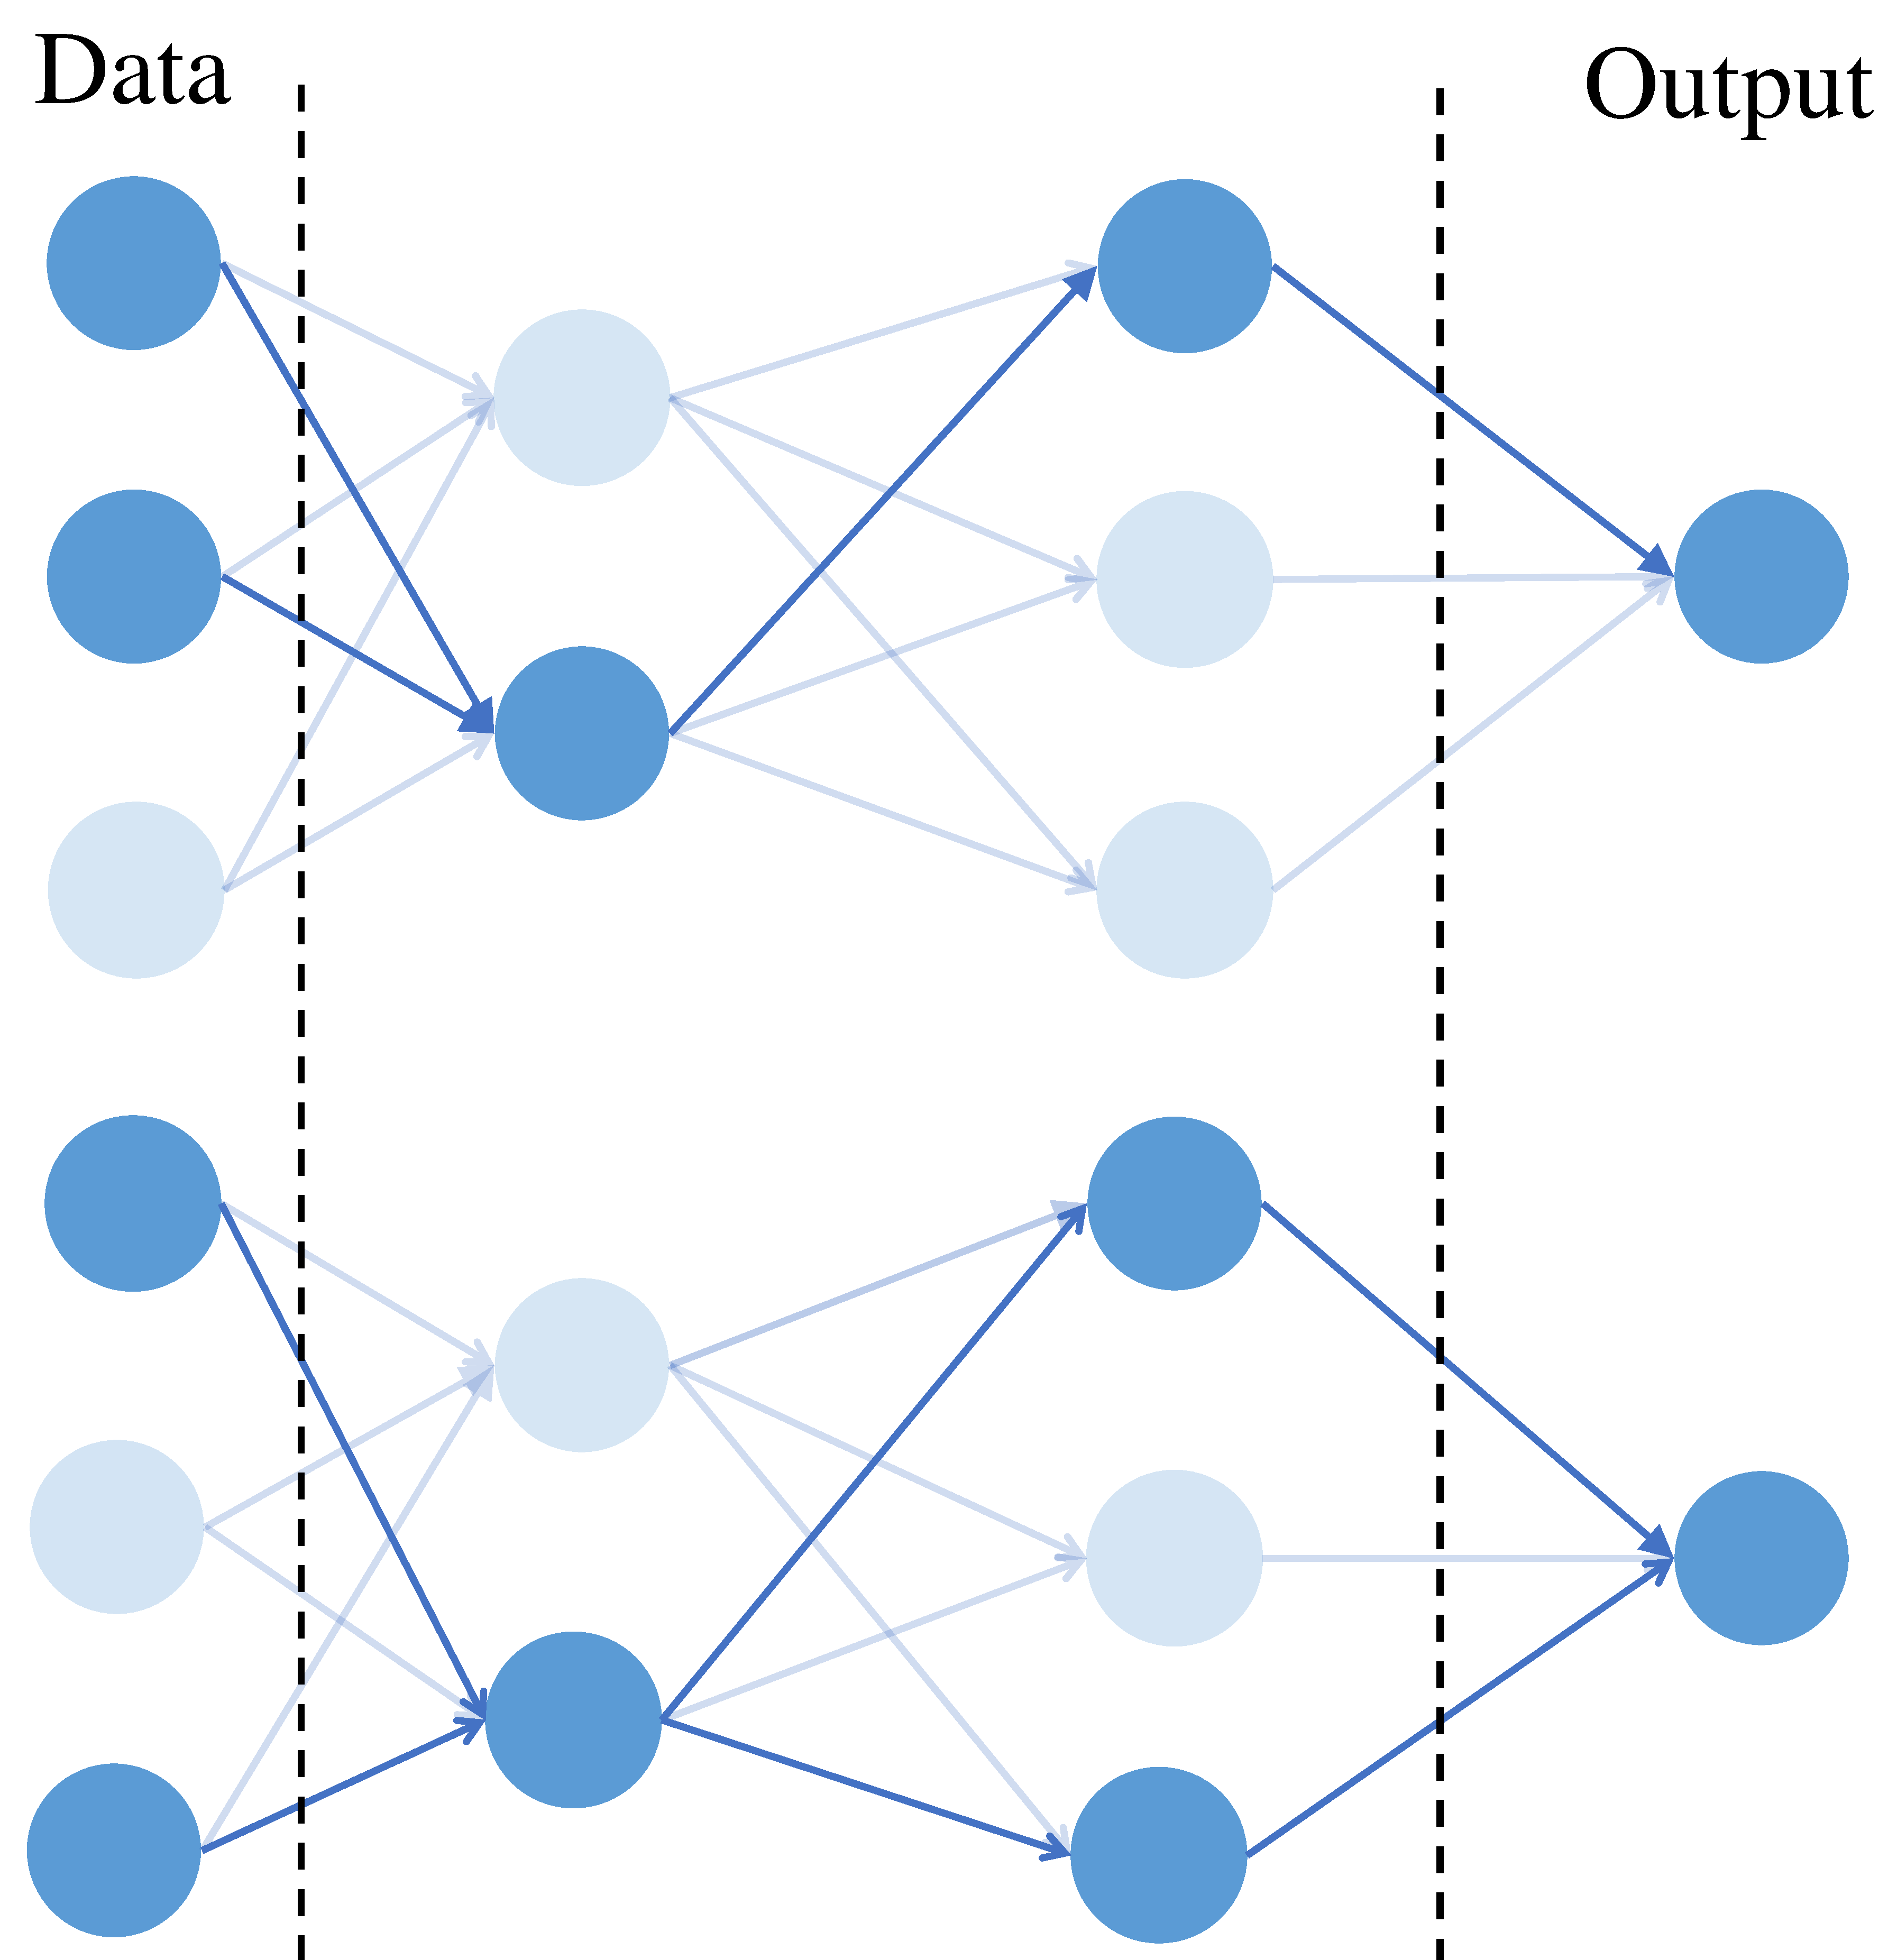
\includegraphics[width=0.45\textwidth]{figures/MonteCarloDropout.pdf}
    \caption{MC dropout的基本结构示意图\cite{DBLP:journals/corr/abs-2011-06225}}
    \label{mc_dropout}
\end{figure}

MC dropout主要捕捉认知不确定性(模型不确定性),这种不确定性体现在
不同dropout掩码下预测结果的变化性上。它可以与预测偶然不确定性的模型结合使用。
不过相比BNN,MC dropout实现更简单,可以方便地应用于已经使用
Dropout进行正则化的现有网络架构;计算成本相比BNN更低。
然而,其贝叶斯近似的质量可能有限;对于大型复杂模型,其不确定性估计可能校准不佳
或不足;而且其性能(包括UQ质量)依赖于dropout率的选择和网络结构;
不确定性的解释可能不够直接。

\subsection{深度集成}

深度集成是训练多个(N个)结构相同(或相似)但参数独立的神经网络模型。\cite{NIPS2017_9ef2ed4b}
这些模型通常使用不同的随机权重初始化,有时也使用不同的训练数据子集
(例如通过bootstrapping,如图\ref{boosttrap}所示)。进行训练。最终预测结果通过组合N个模型的输出得到
(例如,对回归任务取均值,对分类任务取平均概率),而不确定性则由模型预测结果之间的差异
(例如方差)来估计。

\begin{figure}
    \centering
    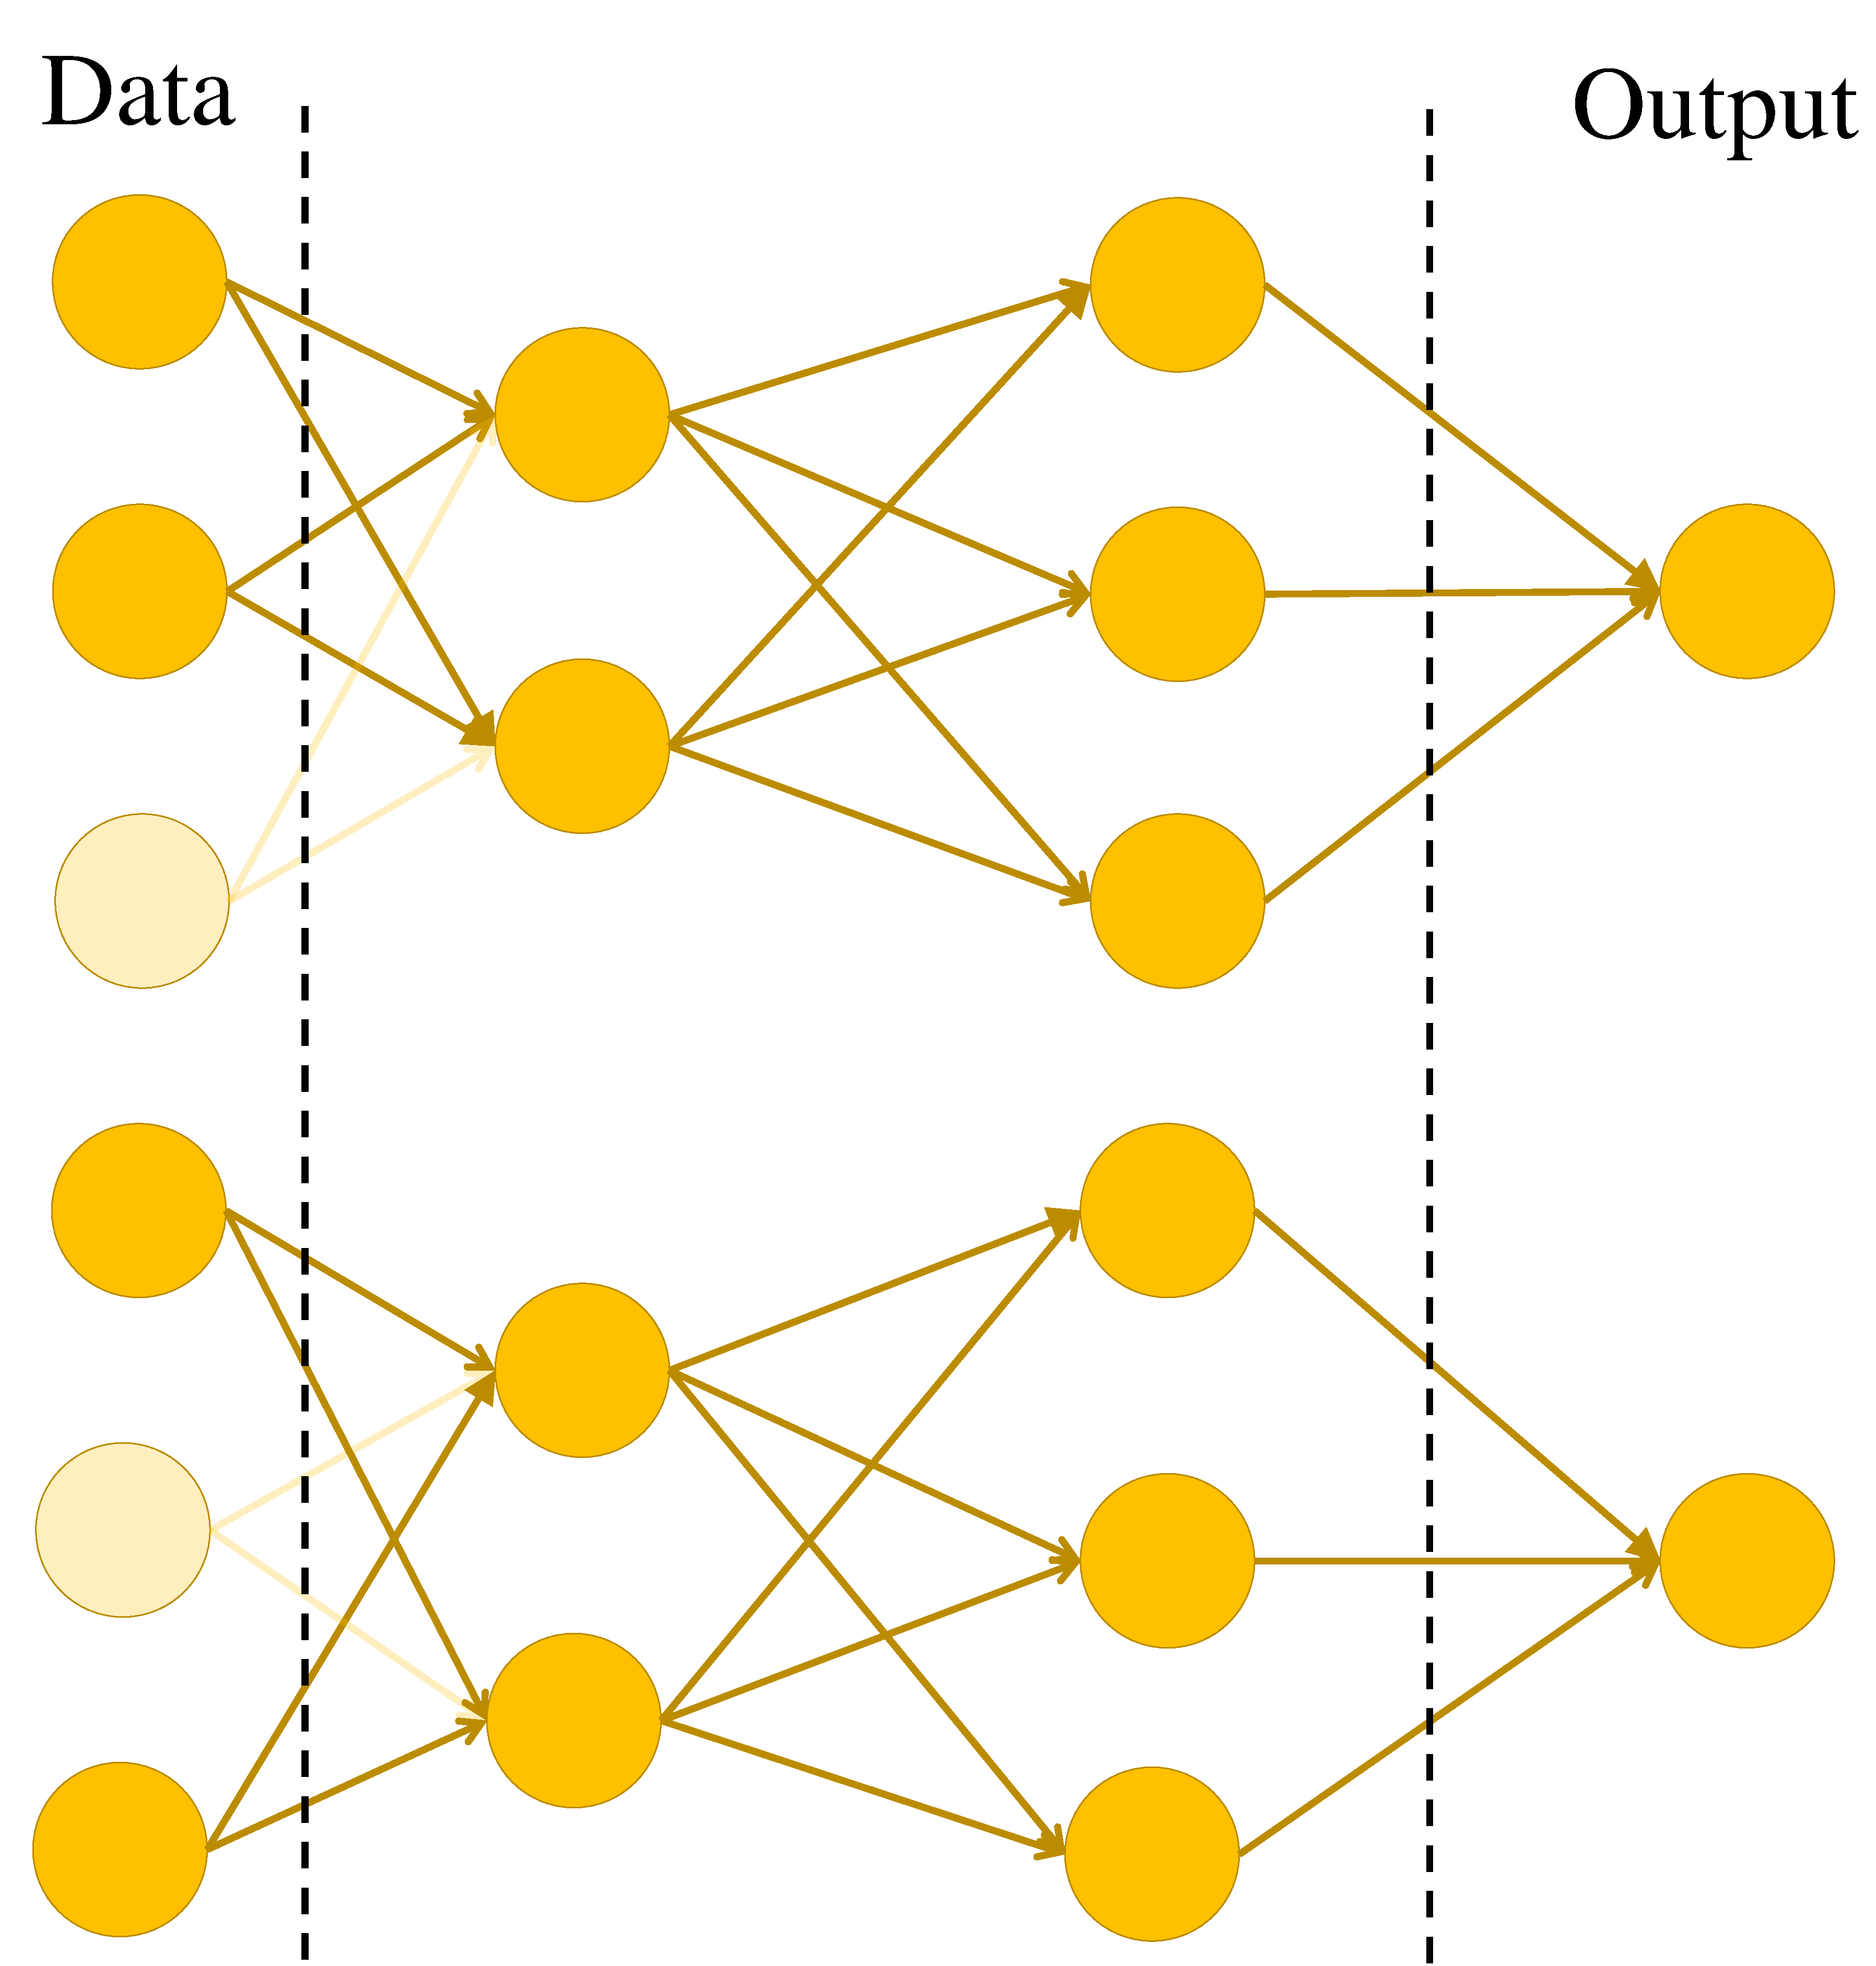
\includegraphics[width=0.45\textwidth]{figures/BootstrapModel.pdf}
    \caption{深度集成训练中Bootstrapping的基本结构示意图\cite{DBLP:journals/corr/abs-2011-06225}}
    \label{boosttrap}
\end{figure}

该方法主要通过模型多样性来捕捉认知不确定性。
可以与能够预测偶然不确定性的模型(例如,预测输出分布的均值和方差)结合,
使用集成预测的方差来估计认知不确定性部分。

深度集成概念简单直观;在许多基准测试和实际应用中,常常能达到顶尖的预测精度和良好的校准性能;
模型训练过程可以并行化;但是训练和推断的计算成本很高(需要训练和运行N个模型),需要大量的存储空间;
同时我们还需要确保集成成员具有足够的多样性;仅仅通过集成预测的差异来估计不确定性,
缺乏严格的数学基础来保证其能可靠地同时涵盖偶然和认知不确定性。

总而言之,不确定性量化在深度学习模型的应用中具有重要意义,
有助于提升模型的可靠性和决策质量。
选择合适的不确定性量化方法需要在计算成本和精度之间进行权衡。

\section{本章小结}

本章首先介绍了一些深度学习的基础知识,从神经网络的基本结构、神经元、激活函数和训练过程等等入手,
同时说明了前馈神经网络的基本原理,并简要提了CNN和RNN等常见变种。
随后,我们重点介绍了在序列数据处理中具有优秀的表现并且获得广泛认可的Transformer模型,
之后详细解释了其核心的自注意力机制,特别是缩放点积注意力和多头注意力。
最后,本章深入探讨了深度学习中的不确定性量化问题,
先对认知不确定性和随机不确定性进行了概念的解释和区分,并详细介绍了三种主流的不确定性量化方法:
BNN、MC Dropout和深度集成。
对每种方法的原理、优缺点和适用场景进行了分析,
强调了不确定性量化对于提升模型可靠性和可解释性的重要性。

